\section{Credit Model Setup}

\subsection{Credit Product Definitions}

This section introduces three core instruments used throughout the project: risky bonds, credit default swaps, and credit linked notes. The goal is to give a clear, intuitive explanation that assumes no prior knowledge of credit markets. We first explain how default works, then show how discount factors and survival probabilities enter the valuation of each cashflow. We break each payoff into simple components and give diagrams that illustrate the structure visually.

\subsubsection*{Default, Recovery, and Survival}

A borrower may default at any time before a bond matures. Default means:
\begin{itemize}
    \item all future coupon payments stop,
    \item the principal is not paid back in full,
    \item instead the investor receives a recovery amount $R$ times notional,
    \item recovery is typically paid immediately when default occurs.
\end{itemize}

If default happens at time $t$, this event has probability density $h(t) Q(0,t)$, where $h(t)$ is the hazard rate and $Q(0,t)$ is the survival probability up to $t$. This explains why recovery terms appear as integrals whereas coupons appear as summations over discrete dates.

Discount factors $P(0,t)$ reduce future cashflows to present value. Survival probabilities $Q(0,t)$ weigh cashflows by the chance that the issuer has not defaulted.

\subsubsection*{Risky Bonds}

A risky bond pays periodic coupons and a principal at maturity, but only if the issuer survives until these dates. If the issuer defaults earlier, coupons stop and the investor receives a recovery payment. We decompose the value of a risky bond into three parts:

\paragraph{1. Coupon leg}
\[
V_{\text{coupon}} = \sum_{i} c\,P(0,t_i)\,Q(0,t_i).
\]

\paragraph{2. Redemption leg}
\[
V_{\text{redemption}} = P(0,T)\,Q(0,T).
\]

\paragraph{3. Recovery leg}
\[
V_{\text{recovery}}
= \int_0^T R\,P(0,t)\,h(t)\,Q(0,t)\,dt.
\]

\paragraph{Total value}
\[
V_{\text{risky}} = V_{\text{coupon}} + V_{\text{redemption}} + V_{\text{recovery}}.
\]

\paragraph{Cashflow diagram}

\begin{verbatim}
Time:   0         t1        t2        ...       T
        |---------|---------|---------|---------|
Cash:     c        c         c         c     +1 (if survive)
Default:           X  ---> Recovery R * Notional
\end{verbatim}

\subsubsection*{Credit Default Swaps}

A credit default swap (CDS) transfers the default risk of a reference entity from one party to another. There are two legs.

\paragraph{1. Premium leg}
\[
V_{\text{prem}} = s \sum_{i} P(0,t_i)\,Q(0,t_i).
\]

\paragraph{2. Protection leg}
\[
V_{\text{prot}} = (1-R)\int_0^T P(0,t)\,h(t)\,Q(0,t)\,dt.
\]

\paragraph{Fair spread}
\[
V_{\text{prem}} = V_{\text{prot}}.
\]

\paragraph{Intuition}
\begin{itemize}
    \item A protection buyer is short credit risk.
    \item A protection seller is long credit risk.
\end{itemize}

\subsubsection*{Identity Linking Bonds and CDS}

\[
\text{Risk Free Bond} = \text{Risky Bond} + \text{CDS}.
\]

This identity shows how the CDS removes the risky bond’s default component.

\subsubsection*{Credit Linked Notes}

A credit linked note embeds a short CDS position into a funded bond:
\[
\text{CLN} = \text{Risk Free Bond} - \text{CDS}.
\]

The coupon is higher because the investor is selling credit protection. CLNs allow institutions that cannot trade derivatives to take credit risk in a funded format.

% =======================================================================
% DETERMINISTIC CURVES
% =======================================================================

\subsection{Deterministic Hazard and Short Rate Curves}

Default risk is represented through a hazard rate $h(t)$, giving survival
\[
Q(0,t) = \exp\left(-\int_0^t h(u)\,du\right).
\]
Similarly,
\[
P(0,t) = \exp\left(-\int_0^t r(u)\,du\right)
\]
gives discounting.

We avoid market calibration and instead specify smooth parametric curves with closed-form integrals.

\subsection{Exponential Hazard and Short Rate Curves}

\[
r(t) = a_r + b_r e^{-c_r t}, \qquad
h(t) = a_h + b_h e^{-c_h t}.
\]

Integrated forms:
\[
Q(0,t) = \exp\Big(-a_r t - \frac{b_r}{c_r}(1 - e^{-c_r t})\Big),
\]
\[
S(0,t) = \exp\Big(-a_h t - \frac{b_h}{c_h}(1 - e^{-c_h t})\Big).
\]

These deterministic curves will become the \textit{initial conditions} for the HJM model.

\subsection{Interpretation of the Parameters}

\paragraph{Long-run level $a$} sets the asymptotic intensity/rate.  
\paragraph{Shift $b$} controls slope at $t=0$.  
\paragraph{Speed $c$} determines exponential decay, equivalently the half-life:
\[
t_{1/2} = \frac{\ln 2}{c}.
\]

\subsection{Chosen Parameters and Economic Motivation}

The project uses simple but realistic parameter sets for the short rate and for two credit qualities: an investment grade (IG) name and a high yield (HY) name. These curves are chosen for plausibility rather than calibration but retain appropriate risk levels and term structure slopes.

\paragraph{Short rate parameters}
\begin{align*}
a_r = 0.02, \qquad b_r = 0.02, \qquad c_r = 0.35.
\end{align*}
This yields $r(0) = 4\%$ and a long run level of $2\%$. The half life is approximately two years. This generates a mild downward slope that is consistent with many developed market environments.

\paragraph{Investment grade hazard rate}
\begin{align*}
a_h = 0.015, \qquad b_h = -0.012, \qquad c_h = 0.30.
\end{align*}
This gives $h(0) = 0.003$ and a long run intensity of $0.015$. The curve slopes upward with a half life near 2.3 years. This matches the pattern of IG credit risk where short horizon default risk is very small but long run uncertainty is higher.

\paragraph{High yield hazard rate}
\begin{align*}
a_h = 0.03, \qquad b_h = -0.02, \qquad c_h = 0.40.
\end{align*}
This yields $h(0) = 0.01$ and a long run intensity of $0.03$. The slope is steeper and the half life is shorter (about 1.7 years). This reflects the behaviour of BB or B rated credits with materially higher default risk.

\subsection{Spread Interpretation Under Recovery}

Under reduced form modelling with recovery of par, the credit spread associated with a hazard rate is
\begin{equation}
s(t) = (1 - R)\,h(t),
\end{equation}
and we adopt $R = 40\%$ which is standard for unsecured corporates.

\paragraph{Investment grade spreads}
\begin{align*}
s_{\text{IG}}(0) &= 0.6 \times 0.003 = 18\ \text{bps}, \\
s_{\text{IG}}(\infty) &= 0.6 \times 0.015 = 90\ \text{bps}.
\end{align*}

\paragraph{High yield spreads}
\begin{align*}
s_{\text{HY}}(0) &= 0.6 \times 0.01 = 60\ \text{bps}, \\
s_{\text{HY}}(\infty) &= 0.6 \times 0.03 = 180\ \text{bps}.
\end{align*}

These spread levels are reasonable for IG and HY credit and support the qualitative interpretation of the chosen parameters.


% =======================================================================
% HJM FRAMEWORK
% =======================================================================

\subsection{HJM Framework for Rates and Hazards}

The deterministic short rate curve $r(t)$ and hazard rate curve $h(t)$ provide the initial term structures of discount and survival. The Heath–Jarrow–Morton (HJM) approach takes these initial curves as inputs and specifies arbitrage-free stochastic dynamics for the entire forward curve. In HJM models the forward curve is the fundamental state variable and all randomness enters through its evolution rather than through the initial term structure.

\subsubsection*{Short Rate, Forward Rate, and Their Relationships}

The short rate $r(t)$ represents the instantaneous risk-neutral interest rate at time $t$. The price of a zero-coupon bond maturing at $T$ is
\[
P(t,T) = \mathbb{E}_t\left[\exp\Big(-\int_t^T r_u \, du\Big)\right].
\]

The instantaneous forward rate $f(t,T)$ is defined by
\[
f(t,T) = -\frac{\partial}{\partial T}\log P(t,T),
\]
which represents the rate applied over an infinitesimal period at time $T$. The short rate is recovered from the diagonal:
\[
r_t = f(t,t).
\]

When $r(t)$ is deterministic,
\[
P(0,T) = \exp\Big(-\int_0^T r(u)\,du\Big),
\qquad
f(0,T) = r(T).
\]
Thus the deterministic short rate curve is equal to the initial forward curve.

\subsubsection*{Hazard Rate, Forward Hazard, and Their Relationships}

The hazard rate $h(t)$ is the instantaneous default intensity. Survival to $T$ is
\[
Q(t,T) = \mathbb{E}_t\left[\exp\Big(-\int_t^T h_u \, du\Big)\right].
\]

The forward hazard rate is
\[
\gamma(t,T) = -\frac{\partial}{\partial T}\log Q(t,T),
\qquad
h_t = \gamma(t,t).
\]

In the deterministic case,
\[
Q(0,T) = \exp\Big(-\int_0^T h(u)\,du\Big),
\qquad
\gamma(0,T) = h(T).
\]
The deterministic hazard curve is therefore the initial forward hazard surface.

\subsubsection*{Initial Forward Surfaces for HJM}

The exponential deterministic curves derived earlier give
\[
f(0,T) = r(T),
\qquad
\gamma(0,T) = h(T).
\]
These surfaces serve as the initial conditions for the HJM evolution.

\subsubsection*{HJM Dynamics and Drift Conditions}

HJM specifies forward dynamics of the form
\[
df(t,T) = \alpha_r(t,T)\,dt + \sigma_r(t,T)\,dW^{(r)}_t,
\]
\[
d\gamma(t,T) = \alpha_h(t,T)\,dt + \sigma_h(t,T)\,dW^{(h)}_t,
\]
with instantaneous correlation
\[
dW^{(r)}_t dW^{(h)}_t = \rho\,dt.
\]

We adopt one-factor exponential volatilities,
\[
\sigma_r(t,T) = \sigma_r e^{-c_r (T-t)},
\qquad
\sigma_h(t,T) = \sigma_h e^{-c_h (T-t)}.
\]

The HJM drift restriction ensures absence of arbitrage. It gives
\[
\alpha_r(t,T) 
= \sigma_r(t,T)\int_t^T \sigma_r(t,s)\,ds
= \frac{\sigma_r^2}{2c_r}\big(1 - e^{-2c_r (T-t)}\big),
\]
\[
\alpha_h(t,T) 
= \sigma_h(t,T)\int_t^T \sigma_h(t,s)\,ds
= \frac{\sigma_h^2}{2c_h}\big(1 - e^{-2c_h (T-t)}\big).
\]

Forward surfaces evolve as
\[
f(t,T) = f(0,T) + \int_0^t \alpha_r(u,T)\,du 
+ \int_0^t \sigma_r(u,T)\,dW^{(r)}_u,
\]
\[
\gamma(t,T) = \gamma(0,T) + \int_0^t \alpha_h(u,T)\,du 
+ \int_0^t \sigma_h(u,T)\,dW^{(h)}_u.
\]

\subsubsection*{Interpretation of Forward Curve Evolution}

The HJM framework models the time evolution of the entire forward curve. The forward rate $f(t,T)$ is defined for maturities $T \ge t$, and at each observation time $t$ the function $T \mapsto f(t,T)$ describes the market-implied instantaneous rates for all remaining maturities. As time increases, both the domain and the shape of this forward curve change.

At time $0$ the full forward curve
\[
f(0,T), \qquad T \in [0,T^*],
\]
is observable from the initial term structure. This curve represents the market-implied future short rates from the present time.

At a later time $t_1$ one observes a new forward curve
\[
f(t_1,T), \qquad T \ge t_1.
\]
The portion of the original curve with maturities $T < t_1$ is no longer relevant because those maturities lie in the past. The short rate at time $t_1$ is obtained from the diagonal through
\[
r(t_1) = f(t_1,t_1).
\]

At a later time $t_2$ the entire curve evolves again,
\[
f(t_2,T), \qquad T \ge t_2,
\]
and both its location and its shape change due to the stochastic HJM dynamics. The curve now begins at the point $T = t_2$, and its behaviour for $T > t_2$ reflects the accumulated randomness up to time $t_2$.

This picture highlights several key properties that are central to HJM modelling.

\begin{figure}[H]
\centering
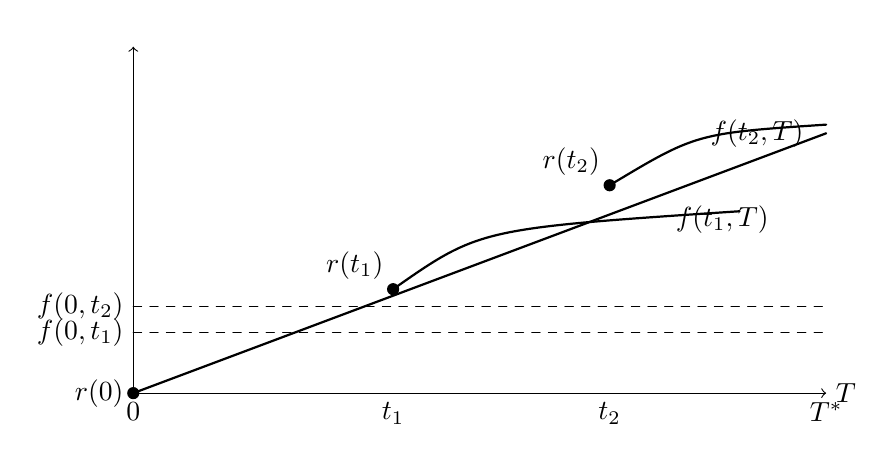
\begin{tikzpicture}[scale=1.1, line cap=round, line join=round]

% Axes
\draw[->] (0,0) -- (8,0) node[right] {$T$};
\draw[->] (0,0) -- (0,4) node[above] {};

% Labels on T-axis
\node[below] at (0,0) {$0$};
\node[below] at (3,0) {$t_1$};
\node[below] at (5.5,0) {$t_2$};
\node[below] at (8,0) {$T^*$};

% Short rate points on diagonal
\draw[thick] (0,0) -- (8,3);

\fill (0,0) circle (2pt);
\fill (3,1.2) circle (2pt);
\fill (5.5,2.4) circle (2pt);

\node[left] at (0,0) {$r(0)$};
\node[above left] at (3,1.2) {$r(t_1)$};
\node[above left] at (5.5,2.4) {$r(t_2)$};

% Forward curve f(0,T) at time 0 (flat dashed)
\draw[dashed] (0,1) -- (8,1);
\node[left] at (0,1) {$f(0,t_2)$};

\draw[dashed] (0,0.7) -- (8,0.7);
\node[left] at (0,0.7) {$f(0,t_1)$};

% Forward curve at time t1
\draw[thick] (3,1.2) .. controls (4,1.9) .. (7,2.1);

% Forward curve at time t2
\draw[thick] (5.5,2.4) .. controls (6.5,3.0) .. (8,3.1);

% Labels for forward curves
\node at (6.8,2.0) {$f(t_1,T)$};
\node at (7.2,3.0) {$f(t_2,T)$};

\end{tikzpicture}
\caption{Evolution of the forward curve. At time zero, the forward curve
$f(0,T)$ is defined for maturities in $[0,T^*]$ and the short rate is $r(0)=f(0,0)$.
At time $t_1$ the forward curve $f(t_1,T)$ is defined for maturities in
$[t_1,T^*]$, and the short rate is $r(t_1)=f(t_1,t_1)$.}
\end{figure}

\begin{itemize}
    \item The forward curve evolves as a random function. At times $t_0$, $t_1$, and $t_2$ the entire mapping $T \mapsto f(t,T)$ shifts according to the dynamics implied by the forward SDE.
    \item The short rate always lies on the diagonal $T = t$ and satisfies $r(t) = f(t,t)$. This identity is fundamental because the short rate drives discounting and appears in all risk-neutral valuation formulas.
    \item As time increases, the region $T < t$ becomes irrelevant. The forward curve is only defined for maturities that remain in the future relative to the current time.
    \item HJM models the full forward curve rather than the short rate. The short rate is recovered from the diagonal, but the dynamics are specified for the entire surface $f(t,T)$.
    \item The simulated object in a Monte Carlo implementation is therefore a curve-valued stochastic process. For every simulation path and every time step, one obtains a full forward curve $f(t,T)$ for all $T \ge t$.
\end{itemize}

These ideas extend directly to the forward hazard surface $\gamma(t,T)$ used for credit modelling. In the CLN valuation framework the HJM dynamics generate stochastic forward hazard curves. At each time step the instantaneous hazard rate is extracted from the diagonal through
\[
h_t = \gamma(t,t),
\]
and this quantity drives CDS spreads, survival probabilities, barrier conditions, optional redemptions, and any payoff components that depend on credit quality. Forward hazard evolution ensures that the expected survival curve matches the deterministic initial curve, which is essential for unbiased Monte Carlo pricing.

Understanding the evolution of the forward surfaces $f(t,T)$ and $\gamma(t,T)$ clarifies the structure of the simulation. It explains why diagonals determine the instantaneous rates, why pathwise integrals of these rates appear in discount and survival factors, and how deterministic term structures propagate consistently into stochastic valuation. This conceptual view forms the link between deterministic credit curves, stochastic forward hazard modelling, and the pathwise hazard rates used in credit-linked note pricing.


\subsubsection*{Bond Prices, Survival, and Instantaneous Rates}

The HJM evolution provides the entire forward surfaces $f(t,T)$ and $\gamma(t,T)$ for interest rates and hazard rates. From these surfaces we recover bond prices, survival probabilities, and the instantaneous short rate and spot hazard rate. These quantities are needed for Monte Carlo valuation of credit-linked notes.

\paragraph{Recovering bond prices and survival probabilities.}

Given forward surfaces at time $t$, the pathwise zero-coupon bond price and survival value are
\[
P(t,T) = \exp\Big(-\int_t^T f(t,u)\,du\Big),
\qquad
Q(t,T) = \exp\Big(-\int_t^T \gamma(t,u)\,du\Big).
\]
These identities hold in both deterministic and stochastic settings. The HJM drift restriction ensures
\[
\mathbb{E}\left[P(t,T)\right] = P(0,T),
\qquad
\mathbb{E}\left[Q(t,T)\right] = Q(0,T),
\]
which guarantees that the simulated curves reproduce the initial term structures in expectation.

\paragraph{Instantaneous rates along the path}

The short rate and spot hazard rate are obtained from the diagonals:
\[
r_t = f(t,t),
\qquad
h_t = \gamma(t,t).
\]
Since negative hazard rates are not meaningful, we apply
\[
h_t \leftarrow \max\{h_t, 0\}.
\]
The accumulated discount factor and survival factor along a simulation path are
\[
D(0,t) = \exp\Big(-\int_0^t r_u\,du\Big),
\qquad
S(0,t) = \exp\Big(-\int_0^t h_u\,du\Big).
\]

\paragraph{Why the pathwise integrals are required.}

Many exotic credit products depend on the instantaneous hazard rate or the cumulative hazard along the path. For example, model-implied CDS spreads satisfy
\[
s_t = (1 - R)\,h_t,
\]
so any payoff referencing credit spreads must use the simulated $h_t$ at each step. Callable and barrier CLNs may depend on the survival value $Q(t,T)$ or on the mark-to-market spread at call dates. Range accrual CLNs often require the hazard rate to remain inside or outside a region.

Even when a payoff depends only on credit quantities, the risk-neutral valuation formula requires discounting through
\[
D(0,t) = \exp\Big(-\int_0^t r_u\,du\Big),
\]
so the short rate must also be accumulated along the path.

\paragraph{Role of the forward SDEs in simulation.}

The forward dynamics
\[
df(t,T) = \alpha_r(t,T)\,dt + \sigma_r(t,T)\,dW^{(r)}_t,
\qquad
d\gamma(t,T) = \alpha_h(t,T)\,dt + \sigma_h(t,T)\,dW^{(h)}_t,
\]
are discretised in time in the Monte Carlo simulation. At each step the entire forward curve is updated, and the diagonal values $r_t = f(t,t)$ and $h_t = \gamma(t,t)$ are extracted. Numerical integration of these processes yields $D(0,t)$ and $S(0,t)$, which drive the pricing of all subsequent CLN cashflows.

The implementation details, including discretisation schemes and variance reduction, are presented in the following section.

